\documentclass[12pt,a4paper]{report}
\usepackage[utf8]{inputenc}
\usepackage[T1]{fontenc}
\usepackage[french]{babel}
\usepackage{graphicx}
\usepackage{hyperref}
\usepackage{listings}
\usepackage{xcolor}
\usepackage{geometry}
\geometry{margin=2.5cm}

\title{Étude comparative entre un serveur TCP mono-thread et multi-thread en C}
\author{Votre Nom}
\date{\today}

\begin{document}
\maketitle
\tableofcontents

\chapter{Introduction}
L'objectif de ce projet est de comparer les performances et le comportement
de deux architectures de serveurs TCP :
\begin{itemize}
    \item un serveur mono-thread, séquentiel, traitant une connexion à la fois;
    \item un serveur multi-thread, basé sur un pool de threads et une file FIFO
          thread-safe pour répartir la charge.
\end{itemize}

Cette étude s'inscrit dans le cadre d'un module de systèmes d'exploitation avancés
et vise à illustrer concrètement les problématiques de concurrence, d'ordonnancement,
de synchronisation, de saturation CPU et de scalabilité.

\chapter{Architecture des serveurs}

\section{Serveur mono-thread}
Le serveur mono-thread est une boucle simple :
\begin{enumerate}
    \item appel bloquant à \texttt{accept()};
    \item réception d'un entier 32 bits;
    \item exécution d'un traitement CPU simulé;
    \item envoi de la réponse (carré de l'entier + timestamp);
    \item fermeture de la connexion.
\end{enumerate}

\section{Serveur multi-thread}
Le serveur multi-thread utilise :
\begin{itemize}
    \item un socket d'écoute unique;
    \item une file FIFO thread-safe bornée;
    \item un pool de workers (8 threads) qui dépilent les sockets clients,
          effectuent le traitement et répondent.
\end{itemize}

Le découplage accept / traitement permet d'exploiter plusieurs cœurs CPU
et de mieux absorber les pics de charge.

\section{File d'attente thread-safe}
La file est implémentée via:
\begin{itemize}
    \item une liste chaînée;
    \item un \texttt{pthread\_mutex\_t} pour protéger l'accès;
    \item deux variables de condition : \texttt{not\_empty} et \texttt{not\_full};
    \item un drapeau \texttt{shutdown} pour un arrêt propre.
\end{itemize}

\chapter{Méthodologie de benchmark}

Le benchmark est réalisé avec un client Python multi-thread qui ouvre
un grand nombre de connexions simultanées (10, 50, 100, 200, 300 clients).
Pour chaque configuration, nous mesurons:
\begin{itemize}
    \item le temps total d'exécution;
    \item la latence moyenne, médiane, P95, P99;
    \item le débit en requêtes par seconde;
    \item l'utilisation CPU et la mémoire RSS côté serveur.
\end{itemize}

Les mesures sont agrégées dans un fichier \texttt{results.xlsx}, puis
visualisées avec des graphiques générés par \texttt{plot\_results.py}.

\chapter{Résultats expérimentaux}

\section{Débit en fonction du nombre de clients}
\begin{figure}[h!]
  \centering
  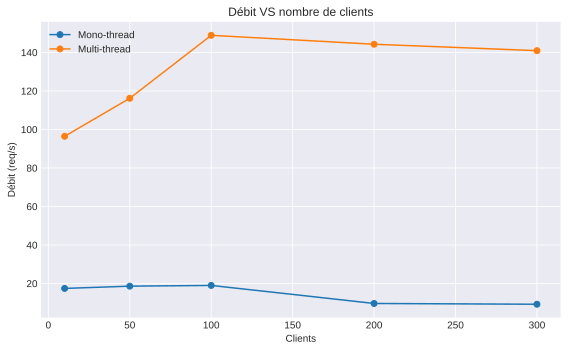
\includegraphics[width=0.8\textwidth]{../python/figures/1-throughput.png}
  \caption{Débit (req/s) en fonction du nombre de clients.}
\end{figure}

\section{Latence P99}
\begin{figure}[h!]
  \centering
  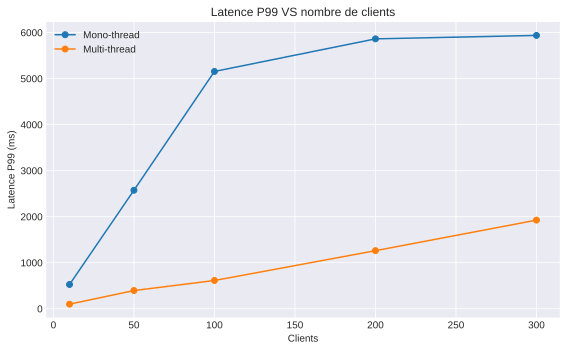
\includegraphics[width=0.8\textwidth]{../python/figures/2-latency_p99.png}
  \caption{Latence P99 en fonction du nombre de clients.}
\end{figure}

\section{Utilisation CPU et mémoire}
\begin{figure}[h!]
  \centering
  \includegraphics[width=0.8\textwidth]{../python/figures/3-cpu.png}
  \caption{CPU moyen en fonction du nombre de clients.}
\end{figure}

\begin{figure}[h!]
  \centering
  \includegraphics[width=0.8\textwidth]{../python/figures/4-memory.png}
  \caption{Mémoire RSS en fonction du nombre de clients.}
\end{figure}

\section{Speedup multi-thread}
\begin{figure}[h!]
  \centering
  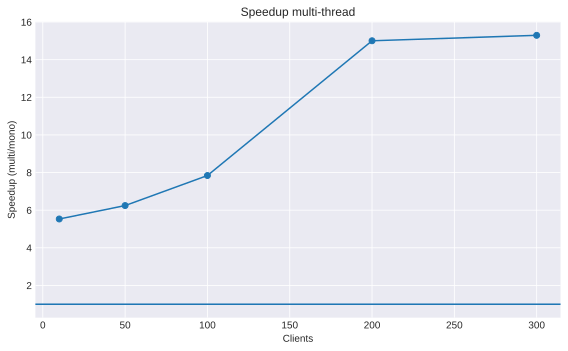
\includegraphics[width=0.8\textwidth]{../python/figures/5-speedup.png}
  \caption{Speedup (multi / mono) en fonction de la charge.}
\end{figure}

\chapter{Analyse et discussion}

Les résultats montrent généralement que :
\begin{itemize}
    \item le serveur mono-thread atteint rapidement un plateau de débit;
    \item le serveur multi-thread continue de monter en charge jusqu'à
          l'utilisation quasi-complète des cœurs CPU;
    \item la latence P99 augmente fortement pour le mono-thread dès que le
          nombre de clients dépasse quelques dizaines;
    \item le multi-thread offre une meilleure réactivité globale, au prix
          d'une complexité de code accrue (synchronisation, file d'attente).
\end{itemize}

D'un point de vue pédagogique, ce projet illustre clairement:
\begin{itemize}
    \item les limites du modèle strictement séquentiel;
    \item les gains apportés par le parallélisme;
    \item les problèmes de contention et de saturation CPU;
    \item l'importance de limiter la taille des queues pour maîtriser la mémoire.
\end{itemize}

\chapter{Conclusion}

Le serveur multi-thread basé sur un pool de threads et une queue bornée
s'avère nettement plus performant et scalable que le serveur mono-thread,
surtout en présence d'une charge importante et de traitements CPU coûteux.

Cependant, cette amélioration de performance s'accompagne d'une complexité
de conception (synchronisation, arrêt propre, gestion des erreurs) qui doit
être soigneusement maîtrisée, en particulier dans des contextes industriels.

\end{document}
